\newpage
\chapter{Approach}
\label{sec:approach}
The role mining problems (see section \ref{sec:roleMiningProblems}) have been approached with different problem formulations, techniques and algorithms. In this thesis the approach of solving role mining with an evolutionary algorithms is investigated.\\
\hl{Evolutionary algorithms seem to be a promising approach for role mining for several reasons.} Role mining is following several objectives, e.g. minimizing the number of roles and minimizing the number of confidentiality and availability violations (over- and underentitlements), which can be in conflict with each other. With multiobjective evolutionary algorithms pareto-optimal solutions, a set of optimal trade-offs solutions, can be found in a single run instead of several runs, which is necessary for some of the conventional stochastic processes, like simulated annealing and tabu search\cite{abraham2005evolutionary}. Previous research in the role mining field are using scalarisation, where several objectives are weighted and summarized in one single objective, like the Weighted Structural Complexity (WSC) in Molloy et al.\cite{Molloy} or the fitness function for the basic RMP in Saenko \& Kotenko\cite{saenko2012design}. The trade-offs between the objectives are not apparent in these approaches.\\
Furthermore the task of role engineering is an on-going process. After an initial role model is created, the user-permission relation can change over time and therefore the roles in the role model can become suboptimal. Evolutionary algorithms can adapt solutions to changing circumstances\cite{Fogel:1997}. A current role model state can be used as starting population and the evolutionary algorithm will optimize towards the formulated objective in the fitness functions.\\
At last role engineering is still a process, which requires human interaction. The role mining results are evaluated by humans and modified to an extend that it is accepted by the business. Interactive evolutionary computation (IEC)\cite{949485} could include human feedback to the algorithm to navigate the evolutionary algorithm to an optimal result. In IEC the fitness function is replaced by an human user.\\\fi

Since there has not been a lot of research done up till now (see chapter \ref{sec:relatedWork} for related work), the research in this thesis starts with a basic set up of the domain-specific problem as evolutionary computation problem. The evolutionary algorithm, the representation of an individual, variation operators, selection mechanisms and fitness functions used in this approach are described in the following sections. \hl{For handling constraints for an RBAC$_2$ role model, a penalty function and intelligent variation operators are introduced. Furthermore the multiobjective evolutionary algorithm used in this approach is described with its challenges and improvements. In order to come to an human digestible representation of individuals for human feedback in an IEC approach, an alternative approach with a different representation and a Co-Evolution technique is presented.}\\
The EA for single objectives is based on the evolutionary algorithm process described in chapter \ref{sec:EA}. A pseudo-code is outlined in Algorithm \ref{alg:EA} in the Appendix.\\
In this thesis a single- and a multi-objective EA for Role Mining has been constructed, where the objectives can be exchanged in regard to the considered Role Mining Problem. In the following the algorithms will be called Evo-RoleMiner and Evo-RoleMiner$M$ accordingly.
    
    \section{Representation of a Role Model as Individual}
    The representation of individuals in an EA is crucial for the success of the EA and influences the variation operators. Finding a good representation of role models as individuals for a Role Mining EA is a challenging task, since the number of roles for a role model is not predefined. In the following one bit-string and two complex representations are introduced and evaluated. The complex representations were proposed by Saenko \& Kotenko\cite{saenko2012design}.
        \subsection{Representation as Bit-string}
        The representation of individuals as bit-string is one of the simplest and is often mistakenly used in genetic algorithms\cite{Eiben}. A suggestion for a bit-string representation for a role model is derived from a combined user-role- (UA) and role-permission-matrix (PA). Figure \ref{fig:representation1} shows an example of a combined UA- and PA-Matrix and an according bit-string representation.
        \begin{figure}[H]
            \centering
            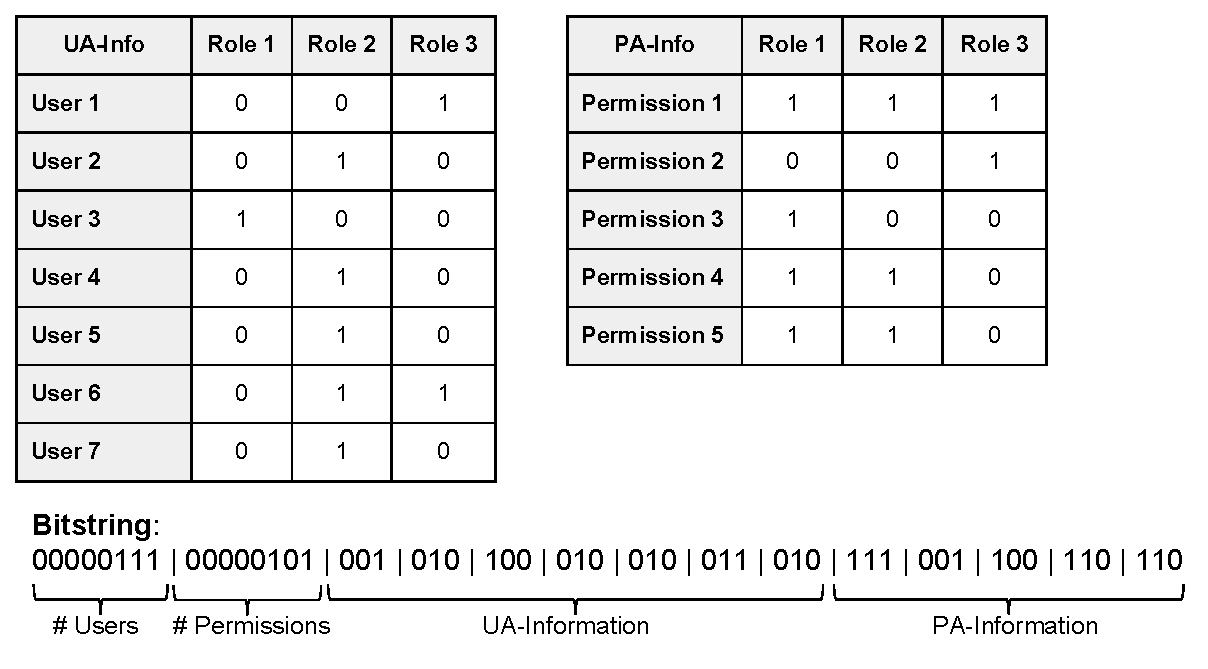
\includegraphics[scale=0.4]{./Figures/BitstringRepresentation}
            \caption{\textit{Example of a UA- and PA-Matrix with its bit-string representation}}
            \label{fig:representation1}
        \end{figure}
        The motivation of this initial idea is that the mutation operator can be easily executed by just flipping a bit within the bit-string. The mutation is therefore adding or removing a user or permission from a role. For the decoding two leading 8-bit integers can represent the number of users and permission. However, the problem with this representation is that the number of roles needs to be pre-defined, such that the bit-string can be decoded again. Alternatively another leading 8-bit integer can represent the number of roles in the role model. But varying the number of roles demands adding or removing bits in the bit-string for each user-role- and role-permission relation. Furthermore the information that a user or a permission is not part of a role seems to unnecessarily lengthens the bit-string, which can consume a lot of space for high-dimensional UA- and PA-Matrices.
        \subsection{Representations as Complex Objects}
        In Saenko \& Kotenko\cite{saenko2012design} two different representations are introduced, which are briefly described in section \ref{sec:relatedWork3}. With the first representation the authors suggest a multi-chromosomal representation where the number of roles becomes part of the search. An example can be seen in figure \ref{fig:representation2}. A drawback of this representation are unnecessary genes (roles) like the unnecessary information in the bit-string representation. Another disadvantage of the representation are complex crossover operations\cite{saenko2012design}.
        \begin{figure}[H]
            \centering
            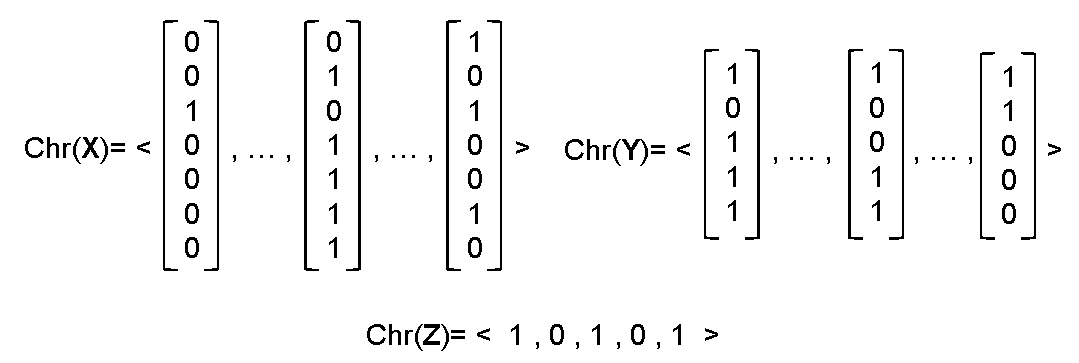
\includegraphics[scale=0.5]{./Figures/ComplexRepresentation1}
            \caption{Example of a multi-chromosomal representation. Chromosome X represents the UA-Informationa and Chromosome Y the PA-Information. Chromosome Z determines if a role is active or passive. The columns in all chromosomes are consistent to roles. In this example roles 1, 3 and 5 are active.}
            \label{fig:representation2}
        \end{figure}
        The second improved representation eliminates these drawbacks by having one chromosome for an individual, where no unnecessary genes (roles) occur. The chromosome consists of a list of roles, which contain a user-list and a permission-list (see figure \ref{fig:representation3}).\\
        \begin{figure}[H]
            \centering
            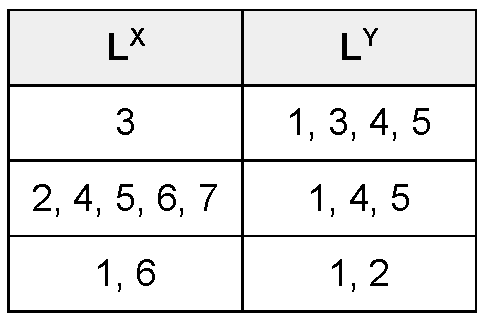
\includegraphics[scale=0.4]{./Figures/ComplexRepresentation2}
            \caption{Example of a role model representation suggested in Saenko \& Kotenko\cite{saenko2012design}. A row represents a role (gene). In the column $L^X$ are user lists and in the column $L^Y$ are permission lists.}
            \label{fig:representation3}
        \end{figure}
        Due to the advantages of the improved representation of Saenko \& Kotenko\cite{saenko2012design}, their suggested representation has been implemented in this thesis. The user- and permission lists are implemented as sets.
    
    \section{Variation Operators on Role Model Representation}
    Dependent on the choice of the representation of individuals in the previous section, according mutation and crossover methods are created. The choice of variation operators and how often they are executed influences how much of the search space is discovered during the evolution. Since the improved representation of Saenko \& Kotenko\cite{saenko2012design} has been selected for this thesis, the following variation operators are suited for this representation.
        \subsection{Mutation methods}
        Since no further instructions for the mutation are given in Saenko \& Kotenko\cite{saenko2012design}, the mutation operations have been chosen intuitively. For the mutation six different mutation types are implemented, which are executed in the following order depending on their probability.
        \begin{itemize}
            \setlength{\itemsep}{1pt}
            \item Add a new role
            \item Add a user to a role
            \item Add a permission to a role
            \item Remove a role
            \item Remove a user from a role
            \item Remove a permission from a role
        \end{itemize}
        Examples can be seen in Figure \ref{fig:mutationOperations}. If an individual gets mutated is determined by a fixed probability $MUTPB$. In addition fixed probabilities for each mutation method is dictating how the individual gets mutated. The probabilities allow to influence how often a certain mutation should be executed and can therefore influence how much new solutions are discovered and how likely good solutions are lost. The mutation operations are implemented in such a way that it is ensured that all users and permissions are assigned to at least one role. This prevents that incomplete role models with missing users or permissions can occur.
        \iffalse Hence the search is restricted to a feasible region\cite{Eiben}.\fi
        \begin{figure}[H]
            \centering
            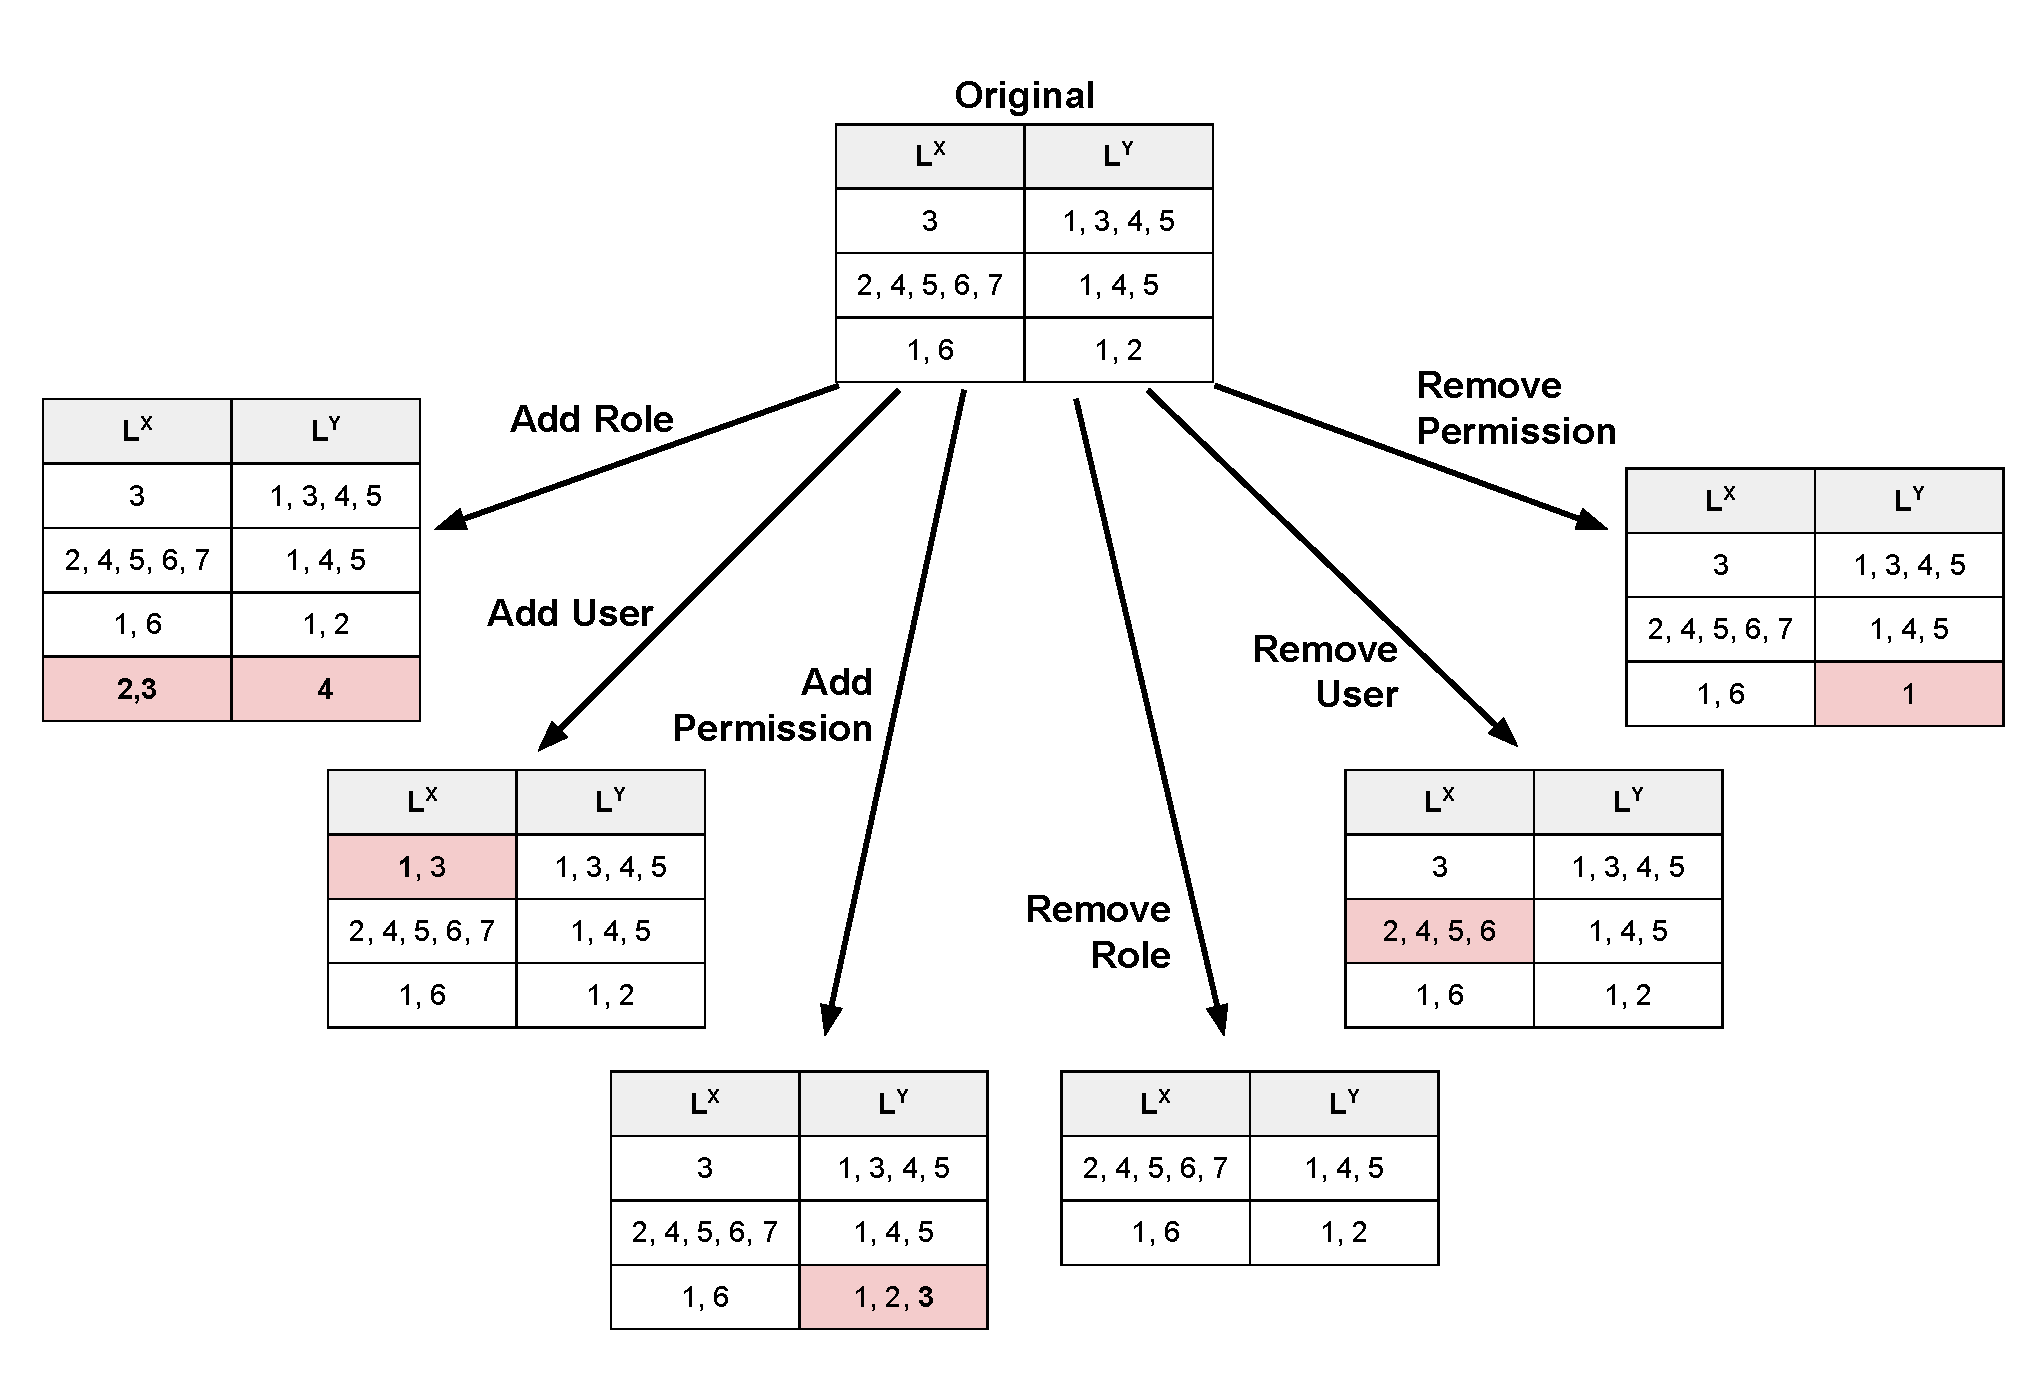
\includegraphics[scale=0.27]{./Figures/Mutations}
            \caption{Examples for the six different mutation operators}
            \label{fig:mutationOperations}
        \end{figure}
        \subsection{Crossover methods}
        The recombination is like in Saenko \& Kotenko\cite{saenko2012design} executed on two individuals with a traditional one-point crossover. Both individuals are keeping their first $x$ roles, while the rest of the roles get exchanged as shown in figure \ref{fig:crossover}. The points of crossover (after $x$ roles) of the two individuals are randomly chosen.
        \begin{figure}[H]
            \centering
            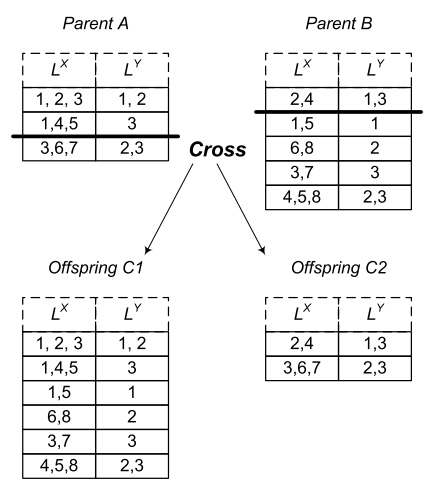
\includegraphics[scale=0.8]{./Figures/crossover.png}
            \caption{Examples of the crossover in the improved GA for the RMP by Saenko \& Kotenko\cite{saenko2012design}}
            \label{fig:crossover}
        \end{figure}
        As for mutation there is also a fixed probability $CXPB$ for crossover operations. It should be noted that the crossover operation can lead to incomplete role models, where users might not get any role or permissions are not contained in any role. While the prevention of incomplete role models is straight forward in the mutation operations, this seem to be less straight forward in the crossover operation.
        \subsection{Local optimization}
        \label{sec:localOptimization}
        A mutation and crossover is always followed by a local optimization on the individual. Like in Saenko \& Kotenko\cite{saenko2012design} the individual is compressed by the rule of User combining and/or Permission combining. If there are roles with the same user sets, they get combined by merging the permissions sets (User combing). Accordingly roles get combined by merging user sets when the same permission sets are present (Permission combining). It should be noted that by this compression the number of roles in the role model can shrink. Furthermore the order of first user combining and then permission combining might not necessarily optimize the individual the best possible way (see example in Figure \ref{fig:localOptimization}b).
        \begin{figure}[H]
            \centering
            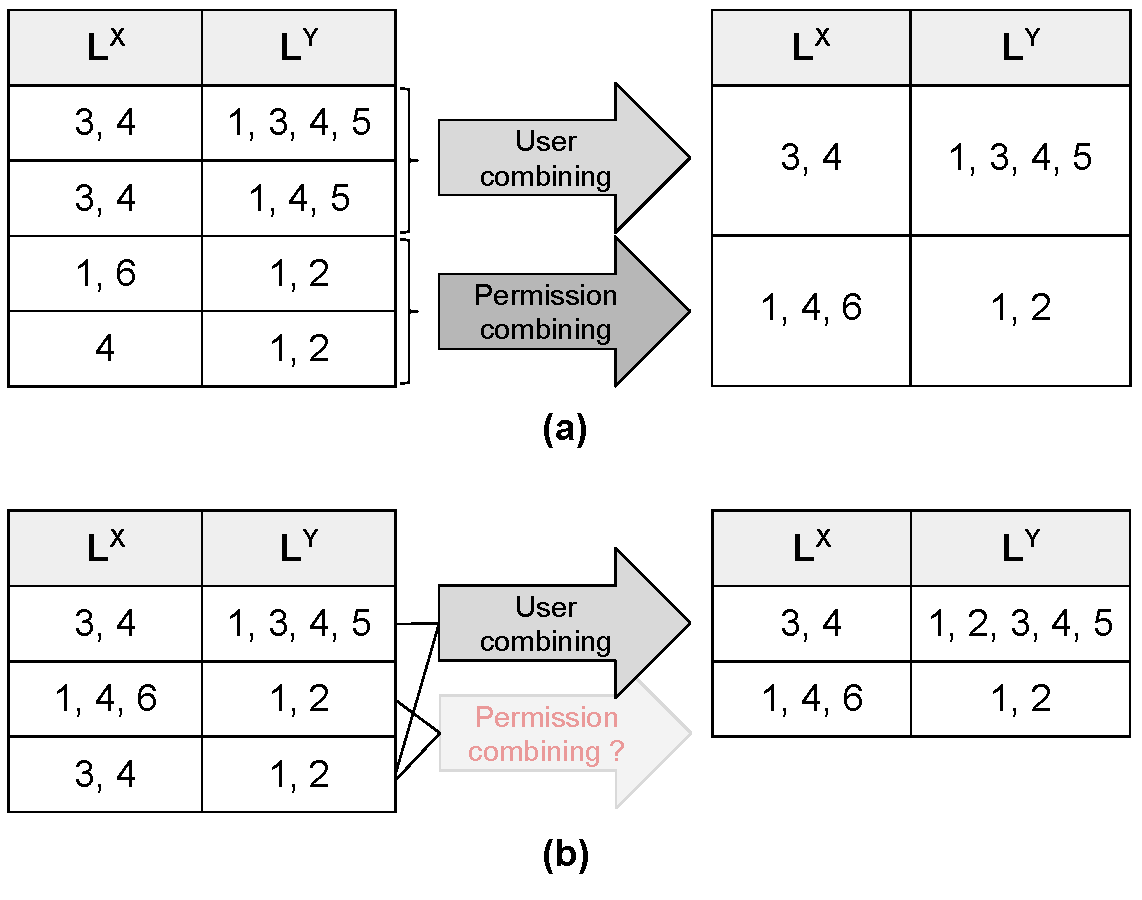
\includegraphics[scale=0.3]{./Figures/LocalOptimization}
            \caption{Examples of local optimizations. In (a) a case for user- and a separate case for permission-combining is detected and executed. In (b) an overlapping user- and permission-combining is detected, but only the user-combining is executed.}
            \label{fig:localOptimization}
        \end{figure}
        
    \section{Selection Strategy}
    Which selection mechanisms are chosen is dependent on if a single-objective or a multi-objective EA is applied.\\
    For the parent selection in the single-objective EA a tournament selection is chosen since it is a widely used selection strategy in EA (see section \ref{sec:parentSelection}). With the tournament size $k$ the selection pressure can be adjusted. The same selection strategy is chosen for the survivor selection in the single-objective EA.\\
    For the multi-objective EAs the selection strategy is dictated by the NSGA-II and NSGA-II$R$ (see section \ref{sec:nsga2} and \ref{sec:crowdingDistance}), where the parent selection is based on a binary tournament selection and the survivor selection is executed on the population of the parent population $P_P$ and the offspring population $P_O$.
    
    \section{Measuring the Interpretability of Roles}
    \label{sec:meaningfulness}
    The goal is to generate a role model, which is accepted by the business, in particular the security administrators. Therefore an appropriate measure has to be found. The interpretability of a role shall express how easy a reasonable interpretation of the role can be identified, such that the role gets adopted by security administrators. An interpretable role is also called a "meaningful" role.\\
    The interpretability of a role in this thesis is measured with the help of user attributes. One or more user attributes can describe the users of a role. For example:\\
    \storestyleof{itemize}
    \begin{listliketab}
        \begin{tabular}{ll}
            Let     &  $OrganizationalUnit \in \{HumanResources, Sales, Motor\}$,\\
                    &  $Location \in \{Denmark, Germany, US\}$ and\\
                    &  $EmployeeType \in \{Internal, External\}$\\
                    &  be the user attributes.  
        \end{tabular}
    \end{listliketab}\\
    The users of a role can be described by an AND-combination of the attribute values, e.g. $Sales \wedge Denmark$ when all users in the role are in $Sales$ and $Denmark$. For simplicity an OR-combination, e.g. $Sales \vee Motor$ where all users would be either in $Sales$ or $Motor$, is not considered. This case can be rather represented by two roles with the same permission-set, but different user-sets. It should be noted that this requires the disabling of the permission-combining optimization (see section \ref{sec:localOptimization}).\\
    \iffalse
    A similar approach is followed in Xu \& Stoller\cite{Xu}, but they calculate an attribute mismatch of roles, which does not consider the heterogeneity of users in different roles as well as homogeneity of users in the same role. In the following sections two approaches are discussed theoretically and one of the approaches is implemented.\\
    \fi
    Two approaches have been considered to measure how well a role can be described by the user attribute values of its user-members. In the following both approaches are introduced, where the later one got implemented.
    
        \subsection{Role Cluster Approach}
        One approach is to treat roles like clusters where the users and their attribute values are objects. A role-cluster is considered good if the user-objects within the role-cluster are compact and the user-objects between role-clusters are separated. This means that the user attribute values considered describe all users within a role (compactness), but no users not in the role (separation). The compactness and separation of a role-cluster can be measured with the average silhouette coefficients of the user-objects of a role-cluster\cite{Han}. If the silhouette coefficient of an user-object approaches 1, the role-cluster, the user is assigned to, is considered compact and the user-object is far away from other role-clusters. A negative silhouette coefficient says that the user-object is closer to user-objects of other role-clusters than to user-objects of the same role-clusters.\\
        This measure of the average silhouette coefficients requires the role-clusters to be crisp, which means a user-object can be only in one role-cluster. But since the users can have several roles the role-clusters are fuzzy. Furthermore the measure has to be executed for every user attribute combination. Therefore an altered calculation of silhouette coefficients has to be used or a different measure has to be used to evaluate the role-clusters. To evaluate fuzzy clusters the sum of the squared error (SSE) can be used\cite{Han}. It measures how well a fuzzy clustering fits a data set. In Rawashdeh \& Ralescu\cite{rawashdeh2012fuzzy} the authors suggest an algorithm for the silhouette coefficient in fuzzy clusters.\\
        The role-cluster approach has not been followed further.
        \subsection{Role Classifier-Rule Approach}
        \label{sec:classifierRule}
        Another approach is to generate classifier-rules for roles and measure the accuracy of these rules. Additionally the rule should be simple and not too complex (e.g. many conditions, which identify exactly one user). For this supervised-learning approach, all users in a role get classified as being in the role, while all other users are classified as being not in the role. Hence for each role a binary classification problem has to be solved. Rules can be extracted from a decision tree or can obtained directly using a Sequential Covering algorithm\cite{Han}. In traditional decision tree construction like ID3 or C4.5 the dataset gets repeatedly splitted based on the attribute which most effectively splits the dataset in one class or the other. The depth of the tree could be used as the complexity measure of a rule. The split by information gain is not necessarily wanted for the rules describing a role, since permissions originally have not been assigned to users which share the most common user attribute values, but rather because users gained legitimation through other specific attribute values. For example although users in a generated role are all located in $Denmark$, while users not in the role are located elsewhere, the reason that users of the role got assigned to the permission set the generated role is grouping could be due to the Departments they are in, which could be diverging. The information gain for the location would be higher, but not necessary the legitimation, why a user gets the permission set assigned through the role. Also the measure used for splitting the data in a decision tree is often biased towards class imbalances or multivalued attributes\cite{Han}. Furthermore classifier-rules for both classes are discovered, while for the measuring of the role only the rules for class "\textit{In the role}" are from interest. Therefore an application-specific algorithm has been created to discover the most descriptive rules for a role (class "\textit{In the role}"). The algorithm got inspired by Sequential Covering algorithms, which directly learns rules for classification by repeatedly removing a portion of the dataset.\\
        The algorithm for rule induction can be seen in Algorithm \ref{alg:ruleInduction}. Before the algorithm is applied on a role, all users of the role in the role model get classified as "\textit{In the role}" or "\textit{Not in the role}". A set of all user attribute combinations is created. If $X$ user attributes are considered, $2^X-1$ combinations are created. For example with the user attributes $Department$ and $Location$, the following combinations are possible:\\
        \centerline{($Department$), ($Location$), ($Department$, $Location$)}\\
        The first user in the role is picked and a the smallest user attribute combination (for example ($Department$)) is chosen. A rule is generated out of the user attribute values of the user for the chosen user attributes. In the example the $Department$ the user is in, creates a rule, i.e. $rule$=($HumanResources$).\\
        Next it will be checked if users not in the role also comply with the rule. If too many users outside the role also comply with the rule, the rule is discarded. Basically the sensitivity of the rule according to class "\textit{Not in the role}" is calculated and checked if it is beneath a specified threshold $t1$ (currently set to $t1$=$\frac{1}{3}$). If the rule persists the check, it is measured how many users inside the role comply with the rule. Again the sensitivity is calculated, but this time on the users in class "\textit{In the role}". If a certain threshold $t2$ is met (currently set to $t2$=$\frac{2}{3}$), the rule is considered as a potential classifier-rule for the role. In this case all users inside the role, which comply with the rule, are not considered any further and are removed. The next user left in the role is picked and a the smallest user attribute combination left (for example ($Location$)) is chosen and the procedure continues as described above until no user attribute combinations or users are left.\\
        User attribute combinations get removed when they are chosen or if a subset of the user attribute combination yields a perfect potential rule, which is when the rule is complying with all users inside the role and with none of the users outside the role. Otherwise a different user combination might yield a better potential rule and is kept as possibility in the user attribute set.\\
        If the threshold $t2$ is not met (percentage of users inside the role comply with the rule is too low), the potential rule gets eventually extended by another OR-connecting rule by calling the procedure recursively. This can be specified by the parameter $max$ in the algorithm. By setting $max$=2 an OR-connecting rule like $Department=HumanResources \vee Department=Sales$ can be constructed.\\
        After generating the rules for a role, the rule with the best accuracy gives the measure for the role interpretability ("meaningfulness"). The accuracy of a rule is measured by
        \begin{equation}
            accuracy = \frac{TP+TN}{P+N}
        \end{equation}
        where:
        \begin{itemize}
            \item $TP$ are the true positives, meaning the number of users classified as "\textit{In the role}" by the rule
            \item $TN$ are the true negatives, meaning the number of users classified as "\textit{Not in the role}" by the rule
            \item $P$ are the true positives, meaning the number of actual users in the role
            \item $N$ are the true negatives, meaning the number of actual users not in the role
        \end{itemize}
        \begin{algorithm}
        	\small
            \caption{Rule induction algorithm for classifier-rules for roles\protect\\
            $D$ = List of role members, which are not matched by current rule\protect\\
            $RM$ = List of users, which are member of the role\protect\\
            $notRM$ = List of users, which are not members of the role\protect\\
            $rule$ = Current rule\protect\\
            $max$ = Maximum allowed rule size (number of OR-connected rules)\protect\\
            $PB_{notRM}$ = Probability that rule matches a user in $notRM$\protect\\
            $PB_{RM}$ = Probability that rule matches a user in $RM$}
            \label{alg:ruleInduction}
            \begin{algorithmic}[1]
                \Procedure{ruleInduction}{$D$,$RM$,$notRM$,$rule$,$max$}
                    \State $allAttrSets$ = Create all combinations of attributes
                    \State sort($allAttrSets$)
                    \State $ruleSet$ = []
                    \While{ $len(D) > 0$}
                        \State $member = D.pop()$
                        \While{ $len(allAttrSets) > 0$}
                            \State $attrSet = allAttrSets.pop()$
                            \State $newRule$ = \textsc{createRule}($attrSet$,$member$)
                            \State $rule$.add($newRule$)
                            \State $PB_{notRM}$ = \textsc{calculateProbabilityInClass}($rule$,$notRM$)
                            \If{ $PB_{notRM} <= (1/3)$}
                                \State $PB_{RM}$ = \textsc{calculateProbabilityInClass}($rule$,$RM$)
                                \State Remove users in $D$, which are matching $rule$
                                \If{ $PB_{RM} < (2/3)$}
                                    \If { $size(rule) <= max$}
                                        \State ... recursion ...
                                        \iffalse
                                        \State $extendedRules$ = ruleInduction($D$,$RM$,$notRM$,$rule$,$max$)
                                        \For {$extendedRule$ in $extendedRules$}
                                            \State $ruleSet$.append($extendedRule$)
                                            \If{ $PB_{RM} == 1$ AND $PB_{notRM} == 0$}
                                                \State $allAttrSets$=\textsc{reduceAllAttrSet}($allAttrSets$, $rule$)
                                            \EndIf
                                        \EndFor
                                        \fi
                                    \EndIf
                                \Else
                                    \State $ruleSet$.append($rule$,$PB_{RM}$,$PB_{notRM}$)
                                    \If{ $PB_{RM} == 1$ AND $PB_{notRM} == 0$}
                                        \State $allAttrSets$ = \textsc{reduceAllAttrSet}($allAttrSets$, $rule$)
                                    \EndIf
                                \EndIf
                            \EndIf
                        \EndWhile 
                    \EndWhile
                    \State \Return $ruleSet$
                \EndProcedure
            \end{algorithmic}
        \end{algorithm}
        
    \section{Fitness Functions for Role Mining Problem Objectives}
    \label{sec:optimizationFunctions}
    Several optimization functions for objectives of the role mining problems (see section \ref{sec:roleMiningProblems}) are separately implemented as fitness functions, such that their impact on the solutions of the Evo-RoleMiner and Evo-RoleMner$M$ can be analyzed. The implemented optimization functions introduced in the following are organized in the according role model categories: Completeness, Complexity and Comprehension (see section \ref{sec:rmQuality}). Finally fitness functions are introduced, which can combine several objectives by scalarisation of the optimization functions. A fitness function is executed on a role model (individual) in the Evo-RoleMiner and Evo-RoleMiner$M$.
        \subsection{Optimization Functions for Completeness}
        \label{sec:optimizationCompleteness}
        To measure the completeness (see section \ref{sec:completeness}) different fitness functions can be created. All of them need the original access control policies $UPA$ for measuring how complete the current considered role model is.
        \begin{itemize}
            \item \textbf{Minimizing Confidentiality Violations}\\
            Confidentiality violations exist when users get more permissions in the generated role model, than they had in the original access control policies (overentitlements). These violations are measured by counting the additional set positive bits ("1") in the resulting matrix of $UA \times PA$ with $UPA$. The worst case of confidentiality violations is the count of all negative bits in $UPA$, meaning that everyone gets all permissions. The best case is to have zero confidentiality violations.
            \item \textbf{Minimizing Availability Violations}\\
            In contrast to confidentiality violations, availability violations exist when users get less permissions in the generated role model, than they had in the original access control policies (underentitlements). Also here the measure is executed by comparing the resulting matrix of $UA \times PA$ with $UPA$, but in this case the negative bits ("0") are counted. The worst case of availability violations is the count of all positive bits in $UPA$, meaning that no one gets the permissions they had in the original access control policies. The best case is to have zero availability violations.
            \iffalse \item \textbf{Minimizing Confidentiality and Availability Violations}\\
            One fitness function is sum of the confidentiality violations and availability violations. Before the values are added, they get normalized. The worst case of availability violations is the count of all positive bits in $UPA$, meaning that no one gets the permissions they had in the original access control policies. The worst case of confidentiality violations is the count of all negative bits in $UPA$, meaning that everyone gets all permissions. For both violation counts 0 is the best case. With the normalization the measures can be weighted, e.g. if availability violations are more acceptable than confidentiality violations, the weight for the later can be bigger.\fi
            \item \textbf{Minimizing Average Confidentiality Violations}\\
            Another fitness function is measuring the average confidentiality violations of roles in a role model. For each role in the role model the overentitlements they are causing in comparison with $UPA$ are counted. In contrast to the fitness function, which is measuring confidentiality violations in the role model, the average confidentiality violations of roles is taken into account that a violation can be caused by several roles.
            \iffalse \item \textbf{Minimizing Average Confidentiality Violations and Availability Violations}\\
            The measure of the average confidentiality violations of roles is combined with the overall availability violations in the role model. As in the other fitness functions, the measures are normalized.\fi
        \end{itemize}
        \subsection{Optimization Functions for Complexity}
        \label{sec:optimizationComplexity}
        To measure the complexity of a role model (see section \ref{sec:complexity}) three different objectives are considered, where no additional information is needed.
        \begin{itemize}
            \item \textbf{Minimizing the Number of Roles}\\
            In the often researched Basic-RMP one objective is the count of roles in the role model, since it is often connected with less administration effort. The goal is to have as little roles as possible. In the used representation of a role model as individual, the number of genes represents the number of roles. The worst case can be determined as having a role for each user or for each permission and is therefore determined as $min(|U|,|P|)$.The best case can be set to one role, although it might be an unrealistic solution.
            \item \textbf{Minimizing the Number of User-Role-Assignments}\\
            In the Min-Edge-RMP the number of User-Role-Assignments and Role-Permission-Assignments have to be minimized instead of the number of roles as in the Basic-RMP. The number of User-Role-Assignments is counted by the positive bits in $UA$. The worst case is if every user is assigned to every role. Since the number of roles can vary, the worst case of the number of roles is considered as number of roles. Therefore the worst case for the number of User-Role-Assignments is $|U| \times min(|U|,|P|)$. The best case is the number of users $|U|$, since each user has at least one permission in $UPA$, which needs to be represented in at least one role.
            \item \textbf{Minimizing the Number of Role-Permission-Assignments}\\
            As mentioned above one of the objectives in the Min-Edge-RMP is the number of Role-Permission-Assignments, which needs to be minimized. The number of Role-Permission-Assignments is counted by the positive bits in $PA$. In the worst case the count is $|P| \times min(|U|,|P|)$, where each permission occurs in each role. The best case is the number of permissions $|P|$, since each permission should be represented in at least one role.
        \end{itemize}
        \subsection{Optimization Functions for Comprehension}
        \label{sec:optimizationComprehension}
        To measure how comprehensive a role model is (see section \ref{sec:comprehension}), a measure had to be found. The approach in this thesis is to measure how "meaningful" the roles of a role model are (see section \ref{sec:meaningfulness}). By having this measure for the role interpretability an optimization function for the objective of comprehension can be formulated as follows. Required is the information of user attribute values, which might not always be at hand.
        \begin{itemize}
            \item \textbf{Maximizing Average Role Interpretability}\\
            The average interpretability of roles in a role model is optimized towards a value of 1. The role interpretability is calculated as described in section \ref{sec:classifierRule}. The worst value is 0, where no descriptive rule for any role in the rolemodel can be found.
        \end{itemize}
        \subsection{Fitness Functions for the Evo-RoleMiner}
        \label{sec:fitnessFunctions}
        Several objectives in the research of role mining are often combined by scalarisation into single objective. The following fitness functions are representing some of these and are combinations of the optimization functions introduced in section \ref{sec:optimizationFunctions}. All objectives get normalized to a value between 0 and 1 before they get into a combined fitness function.
        \begin{itemize}
            \item \textbf{Fitness Function for the Basic-RMP}\\
            In Saenko \& Kotenko\cite{saenko2012design} a weighted function is suggested which takes the number of roles, confidentiality violations and availability violations into account. The function represents the objectives of the basic RMP. The authors formalize the function as maximization function:
            \begin{equation}\label{eq:FBasic}
                F_{basic} = (w_1 * |R| + w_2 * G^{conf} + w_3 G^{accs})^{-1}
            \end{equation}    
            where $G^{conf}$ are the number of confidentiality violations and $G^{accs}$ the number of availability violations. With the weights $w_i$ the influence of the single objectives can be adjusted. A similar fitness function is created, but formalized as Minimization Function:
            \begin{equation}\label{eq:FBasicMin}
                F_{basic}^{min} = w_1 * |R| + w_2 * G^{conf} + w_3 G^{accs}
            \end{equation}
            For the Evo-RoleMiner the Minimization function is used since the math operation to turn the fitness function into a maximization function is unnecessary for the outcome of the result and has only a negative influence on the time performance. This has been also confirmed by running ten experiments for the fitness functions in \eqref{eq:FBasic} and \eqref{eq:FBasicMin} each.\hl{see appendix}
            \item \textbf{Fitness Function for the Min-Edge-RMP}\\
            Another commonly used objective function, the Weighted Structural Complexity (WSC)\cite{Molloy}\cite{Xu} has been used as implementation guideline. Since a role hierarchy (see section \ref{sec:rolehierarchies}) is not in the scope of this thesis, the WSC used is without the number of role-to-role inheritance relations. The WSC is therefore defined as:
            \begin{equation}
                WSC(\gamma,W) = w_1 * |R| + w_2 * |UA| + w_3 * |PA| + w_4 * |DUPA|
            \end{equation}
            where $\gamma$ is the role model and $W$ a set of weights. It should be noted that $DUPA$ are the direct assignments to reduce availability violations. Since the results would lead to a lot of overentitlements, the objective of confidentiality violations is added to the function. The new function is described as:
            \begin{equation}\label{eq:WSCStar}
                WSC(\gamma,W)^* = w_1 * |R| + w_2 * |UA| + w_3 * |PA| + w_4 * G^{accs} + w_5 * G^{conf}
            \end{equation}
            where $\gamma$ is the role model and $W$ a set of weights. When the function in \eqref{eq:WSCStar} was tested with different weights it showed that the number of roles got reduced quickly over the generations, although $w_1$ was set to 0 or lower. By looking at the optimization function description for User-Role- and Role-Permission-Assignments (see section \ref{sec:optimizationComplexity}) it is obvious that the number of roles already gets its impact through the number of User-Role- and Role-Permission-Assignments. When removing the first summand from \eqref{eq:WSCStar} the function is similar to the function in Saenko \& Kotenko\cite{Igor} for the Min-Edge-RMP, which is defined as maximization function:
            \begin{equation}\label{eq:FEdge}
                F_{edge} = (w_1 * (|UA| + |PA|) + w_2 * G^{conf} + w_3 * G^{accs})^{-1}
            \end{equation}
            where $w_i$ are the weights for the single objectives. Hence the maximization function in \eqref{eq:FEdge} is used as guideline for a minimization function for the Min-Edge-RMP: 
            \begin{equation}\label{eq:FEdgeMin}
                F_{edge}^{min} = w_1 * (|UA| + |PA|) + w_2 * G^{conf} + w_3 * G^{accs}
            \end{equation}
            where $w_i$ are the weights for the single objectives. The Minimization function is used for the Evo-RoleMiner for the same reason why the minimization function is chosen in the Basic-RMP: The conversion into a maximization function does not influence the result and has only a negative influence on the time performance.
            \item \textbf{Fitness Function for the Interference-RMP}\\
            At last the objective for comprehension is combined with the objectives of completeness and complexity. The interpretability measure is added to the fitness functions of the Basic-RMP and the Min-Edge-RMP.
            \begin{equation}\label{eq:FBasicMin_INT}
                F_{basic\_INT}^{min} = F_{basic}^{min} + w_6 * (1-INT)
            \end{equation}
            and
            \begin{equation}\label{eq:FEdgeMin_INT}
                F_{edge\_INT}^{min} = F_{edge}^{min} + w_6 * (1-INT)
            \end{equation}
            where $INT$ stands for the interpretability measure and $w_6$ is the weight for the interpretability objective. Since the function is a minimization function, the Interpretability value is inversed in order to reward a higher interpretability.
        \end{itemize}
    
    \section{Initialization of the Population and Termination condition}
    The initial population is randomly generated by creating chromosomes (role models) of random gene size (role size), which contain a random set of users and permissions. It is ensured that each role has at least one user and permission assigned. It should be noted that incomplete role models can be generated, where users might not get any role or permissions are not contained in any role.
    
    \section{Constraint Handling for RBAC$_2$ role models}
    \hl{SECTION UNDER CONSTRUCTION}\\
    In the RBAC$_2$ model (see section \ref{sec:rbac2}) constraints like SoD are taken into account. These can be used to guide the role engineering process, such that constraint violations are not occuring in the role model. Alternatively constraints violations in the role model can be accepted in the role model and are the constraints are complied in a post-mechanism.\\
    The concept of penalties in EA seem to be a good fit to easily incorporate constraints in the Role Mining EA. A binary penalty function would distinguish between if an individual (role model) would violate a constraint or not. Individuals (role models) are therefore penalized with a bad fitness if they are not feasible (violating a constraint).\\
    A distance-based penalty function would measure how difficult it would be to repair the solution.\\
    \hl{implementation not completed}
    
    \section{Multi-Objective Evolutionary Algorithm "Evo-RoleMiner$M$"}
    \hl{SECTION UNDER CONSTRUCTION}\\
    To analyze the different objectives a MOEA has been implemented. The NSGA-II algorithm is applied and reveal the algorithm is not good in handling individuals with the same fitness. The Fortin improvement is applied. Since the objective of number of roles has a too strong impact, a NSGA-II algorithm with weights is implemented.
        \subsection{NSGA2}
        Why? The higher the role number (1 Role for each user), the more likely it is to have no violations. The lower the role number, the more violations
        \subsection{Improved NSGA2}
        Fortin
        Why? Different Individuals have same fitness
        \subsection{Weighted NSGA2}
        Why? 2nd objective is less important\\
        Issue? Skipped fronts, no symmetry in domination matrix

    \section{Alternative Approach with Co-Evolution}
    \hl{SECTION UNDER CONSTRUCTION}\\
    Instead of that individuals represent RBAC models, the individuals represent roles. The motivation behind this approach is to involve human interaction in the survival selection of the EA. Since a whole RBAC model can be hardly evaluated at once, the individuals have to be a smaller fraction of the RBAC model.
        \subsection{Representation of a role as individual}
        \subsection{Variation Operators on role representation}
        \subsection{Symbiotic, Adaptive Neuro-Evolution (SANE)}
